\documentclass[11pt]{article}

\usepackage{geometry}
% Math formatting
\usepackage{amsmath}
\usepackage{amssymb}

\usepackage{longtable}

% Lay out packages
%\usepackage[margin=3.5cm]{geometry}
\usepackage[utf8]{inputenc}
%\usepackage{mathpazo}

% More compact bibliography
\usepackage{natbib}
\setlength{\bibsep}{0.0pt}

% Dutch style of paragraph formatting, i.e. no indents. 
\setlength{\parskip}{1.3ex plus 0.2ex minus 0.2ex}
\setlength{\parindent}{0pt}
\usepackage[protrusion=true,expansion=true]{microtype}

% Command for Horizontal lines
\newcommand{\HRule}{\rule{\linewidth}{0.5mm}}
% Command for degree symbol
\newcommand{\degree}{\ensuremath{^\circ}}

% Add images and pdf pages
\usepackage{graphicx}
\usepackage{pdfpages}

% Colored rows in tables
%\usepackage[table]{xcolor}

% Clickable links with hyperref package
\usepackage[pdfborder={0 0 0 0}, linkcolor=black, urlcolor=blue]{hyperref}

% Fancy Header
\usepackage{fancyhdr}
\pagestyle{fancy}

% Nicer tables
\usepackage{booktabs}
\newcommand{\ra}[1]{\renewcommand{\arraystretch}{#1}}


% Psuedo code
\usepackage{algorithm}
\usepackage{algorithmic}

\rhead{\large\bfseries Gamification and Learning Analytics for Education} % right header: document title
\lhead{\textsc{Jurriaans}, \textsc{Latour}} % left header: document author
\cfoot{\large \thepage} % center footer: page number

\setlength{\headheight}{18pt}

\setcounter{tocdepth}{1}

\begin{document}

\begin{titlepage}
\begin{center}

\includegraphics[width=1\textwidth]{img/uva}\\[1cm]
\HRule \\[0.4cm]
% Title
Exploring the Possibilities of Applying Gamification and Learning Analytics to Education \\A Literature Research \\[0.4cm]
\HRule \\[1cm]
\begin{tabular*}{0.95\textwidth}{@{\extracolsep{\fill}} l r}
Robrecht \textsc{Jurriaans} & Sander \textsc{Latour} \\
\textsc{5887380} & \textsc{5743044}
\end{tabular*}

\vfill \today
\end{center}
\end{titlepage}

\newpage
\thispagestyle{empty}
\mbox{}
\pagebreak

\pagestyle{empty} %get rid of header/footer for toc page

\tableofcontents
\addtocontents{toc}{~\hfill\textbf{Page}\par}

\begin{abstract}
	
\end{abstract}


\cleardoublepage %start new page
\pagestyle{plain} % put headers/footers back on
\setcounter{page}{1} %reset the page counter


\section{Introduction}
% Introduce the current status of education and the problems that lie with motivation
There is an ongoing desire to improve study success in higher education.
Work has been done to identify students that have a high risk of dropping out. (refs)

Two factors in study success seem to be 1) the match between the level of the student and the level of the courses' materials and 2) the student's engagement and motivation.

Students often come from different backgrounds and 

\cite{Horizon2012}

% Use psychological evidence to determine key-factors in motivation and how it improves learning


% Introduce Gamification and Learning Analytics as solutions to this motivation problem



% Research Questions


% Overview of Paper

\section{Gamification}
Games are unprecedented in motivating and engaging players. Humans tend to spent large amounts of time playing games of all sorts. This led some people to believe that it could be possible to generate this type of motivation and engagement in other contexts as well by applying the underlying game design patterns to areas other than gaming to steer behaviour.

Gamification is a concept that is both controversial \cite{McGonigal2011} as well as hard to define \cite{Deterding2011}. The controversy of the term gamification is easily seen in the many different terms that have been coined, including pervasive games, alternate reality games, productivity games, applied gaming, etcetera. All of these terms refer to the practice of applying game design patterns to non-gaming contexts to achieve higher motivation and engagement from users. The term gamification originates from 2004 when it was first used by Nick Pelling as a marketing term \cite{Huotari2012}. In recent years, gamification has moved beyond being just a marketing technique and becoming an academic field. The mayor problem with gamification is that the definition is very subjective and it is difficult to formalize the definition \cite{Huotari2012, Deterding2011}. 
%
The definition of Gamification given by Deterding is:
\begin{quote}
	``Gamification'' is the use of game design elements in non-game contexts. 
\end{quote}

The two important concepts in this definition are ``game design elements'' and ``non-game contexts.'' ``Game design elements'' or ``game atoms'' \cite{Deterding2011, Brathwaite2008} are elements that are not unique to games, but instead are used often in ``gaming contexts''. Such elements can be the state, the dynamics, theme, goals and mechanics of a game and the player and his avatar. The definition for game elements is also subjective as any of these elements can be used outside of the game-context or ``magic circle of games'' \cite{Huizinga}. To give a formal definition of game-elements we would first need to define game-contexts.

Another definition for gamification is given by Huotari et al \cite{Huotari2012} which is from a marketing point of view.
\begin{quote}
	“(Gamification is a) service packaging where a core service is
enhanced by a rules-based service system that provides feedback
and interaction mechanisms to the user with an aim to facilitate
and support the users’ overall value creation.”
\end{quote}

Deterding challenges this definition by addressing that a rule-based system covers more than just games \cite{Deterding2011}. Furthermore, by viewing gamification only from a service marketing perspective does not fully take the social and experiential dimensions of games into account. Nevertheless, both definitions see gamification as the introduction of game-like elements into non-gaming contexts.

Non-game contexts is a broad term for anything that is not a game in itself. However, non-game contexts may also apply to games themselves \cite{Deterding2011}. Parts of the game that may not necessarily be part of the design of the game can be considered as non-game contexts. These type of meta-games have been considered as separate from the game design itself. The game-context is thus also difficult to capture in a formal definition as games can be considered to be something subjective by nature. 

In game theory, games are formally defined as a set of players or agents, a set of moves or strategies and a pay-off function or reward system. In this definition the game elements are already considered as being the set of moves and the reward function. The reward function would then hold all the underlying game mechanics whereas the set of moves can be interpreted as the user interface. For a gamification framework we would like to be able to understand more about the elements that fall under reward functions and the set of moves, as there is common notion that gamification is more then adding rewards and available moves to a non-gaming context.

\subsection{Game Elements}
Byron and Reeves \cite{Byron2009} consider game-elements to be any part of a game and give a list of game elements that help to make a game more engaging. These game elements are: Self-representation with avatars; three-dimensional environments; narrative context; feedback; reputations, ranks, and levels; marketplaces and economies; competition under rules that are explicit and enforced; teams; parallel communication systems that can be easily configured; time pressure. These elements differ from the set of moves and the reward function as found in game theory. Although elements such as feedback and ranks seem to be correlating to intrinsic rewards and thus the reward function, avatars and communication systems appear to be different from this as they are actions that do not directly influence the pay-off.

% Ontology project
Another way of viewing game contexts and game elements is by creating an ontology such as the Game Ontology Project (GOP) \cite{Zagal2008} which is a framework for describing, analysing and studying games. It is a hierarchy for defining games using prototype theory and grounded theory to account for a growing and changing field of games. The ontology is based around four main categories: Interface; Rules; Entity Manipulation and Goals. The interface category comprises how a player interacts with the game, which comprises of both perception and user input. The rules are the rules in the game that work apart from the player, such as the physics, as well as direct consequences of user actions. This latter category seems to be related to the category of entity manipulation, but the main difference is that in the rules category, user actions affect certain underlying mechanics, whilst user actions affecting entities within the rule system belong to entity manipulation. The final category goals holds all the 
information about the direction of the game: when the game ends; how the score is calculated and the actual goals for the player.
These game elements are on a higher level than the game elements as described by Byron and Reeves \cite{Byron2009}, but are on a lower level than the game theory description of games. This ontology is based on the notion that game elements represent smaller chunks of gameplay \cite{Zagal2009} and thus the Game Ontology Project is mainly focused on gameplay elements.

% Game classification elements
A slightly different ontology is given by Elverdam \cite{Elverdam2007} which is based on the Typology Model of games. It is mainly used for the classification of games and works by separating the general concepts: Physical Space; Virtual Space; Internal Time; External Time; Player Relation; Player Composition; Struggle and Game state. Although the model is used for classification as opposed to generation or game design, it is still capable of describing the various game elements. It is a model which is geared towards separating the various types of game design patterns without giving actual separate game elements, but rather categories of game elements which are present in game-play. The eight different categories can be categorised on a higher level as: Players; Space; Time and Rules. These categories differ from the Game Ontology Project in that it is more focussed on the type of game as opposed to the inner mechanics of the game.

% Game design patterns
A similar approach is used by Bj\"ork et al \cite{Bjork2003, Bjork2003b} where game genres are used to derive game design patterns consisting of combinations of game elements. Game elements are seen as components that are used often within certain genres. The components are categorised into four distinct categories: holistic, bounding, temporal and structural. Holistic components are the elements that define how the game differs from other activities and how players can join a session and how the game session ends. Such components include the game instance, game and play session, set-up and set-down activities and extra-game activities. Unlike holistic components, bounding components describe the purpose of the game and what activities are allowed within the game context, these include the rules, the goals and sub-goals and the modes of play. The temporal components are those elements that divide the complete game session into smaller sessions such as the individual actions, events, closure or the end of 
such a session and the evaluation at the end. The structural components are the components that are interacted with and manipulated by the players. This category includes the players and their avatars, the interface and game elements. The terminology is different from the game elements as discussed before, which overlaps with the components as described by Bjork et al. Here the game elements represent entities within the game context that inform the players about the current game state.


%% Game contexts
% Magic circle of play
As the literature shows, game elements are usually defined as being design patterns used in game design. The game elements are elements that can be found in game contexts, although the definition of the game context is different depending on the task of the ontology. When classifying games, the game elements that are used are based on different genres, while for game design, the game elements are used as experience-design patterns. There seems to be no definite set of game elements for all purposes as some of the elements change context determined by the task of the ontology. So to define a set of game elements, it is important to first understand what constitutes as a game context. 

\subsection{Game Contexts}

In Huizinga's ``Homo Ludens: A Study of the Play-Element in Culture'' \cite{Huizinga} the play context is described as being a ``Magic'' circle. The magic circle is a concept that is used, in a similar fashion to assemblage theory \cite{Taylor2009}, to denote all elements within a certain contextual domain. The circle refers to a contextual domain that is either materially or ideally marked off and contains all elements that are relevant to the domain. The strength of this concept lies in that it allows for any domain to be viewed as being a circle for play. While Huizinga refers to this as a circle for play, the concept was later applied to digital games by Salen and Zimmerman \cite{Zimmerman2004}. In the context of a game, the magic circle is the domain that is entered when a player starts a game and thus all elements that are relevant during the game are the game elements of that game.

This notion of a magic circle is vastly different than the view of games as being interactive narratives \cite{Hartsook2011,Marchiori2011,Li2012,Jenkins2004}. Seeing games as interactive narratives creates the opportunity to compare games with more traditional story-telling such as writing, films and even static art. Many genres of games also overlap between traditional storytelling and games, such as interactive novels and role-playing games. However, not all types of games fall into this classification in a natural manner. When playing chess, not many people will be bothered with an actual story about warfare. Some of these games have a different type of narrative that breaks away from a traditional story and are more the narrative or experience of the game. For instance, tic-tac-toe does not have a proper story, but playing it creates a narrative between the players engaged in the game.

% Experiential Flow
Another method of describing games is as the mental state that games trigger in players \cite{Kiili2005} called the experiential flow. This flow is segmented into three distinct parts: Antecedents, Flow experience, Flow consequences. The antecedents are the actual game setting represented as the person, the task and the artefacts. These three components interact which causes the player to get the flow experience. This experience has various effects on the player including time distortion, merging of action and awareness, concentration, telepresence, sense of control and the loss of self-consciousness. Due to these effects the player then experiences the flow consequences. These flow consequences are indirect effects on the player such as improved learning, changes of attitude, exploratory behaviour and perceived behavioural control.

In the book \emph{Andrew Rollings and Ernest Adams on Game Design} \cite{Rollings2003} the definition of a game is derived from the informal definition as given by game designer Sid Meyer.
\begin{quotation}
	[Gameplay is] a series of interesting choices
\end{quotation}

With this quote, Sid Meyer touches upon what lies at the heart of a game and what Huizinga described as the magic circle. Games are defined by their gameplay in a sequence of events held together in the assemblage of the domain. The definition is made more formal by defining the "interesting choices." 

\begin{quotation}
	[Gameplay is] One or more causally linked series of challenges in a simulated environment \cite{Rollings2003}
\end{quotation}

The big difference is with Sid Meyer's original quote is the naming of the simulated environment and the alteration of the interesting choices to a series of challenges. The game is now defined by one or more linked series of challenges which represent the different types of gameplay that can be present in a game. These causal links are closely related to assemblage theory and the magic circle. The challenges not only refer to the gameplay being an actual challenge, but more to certain events and obstacles that the player has to overcome to reach the goal of the game.


\subsection{Application of Gamification}



\subsection{Game-based Learning}




\section{Learning Analytics}
%introduction
There is an ongoing whish to increase study success of students in higher education. Stakeholders demand educational institutions to make data-driven decisions to improve perfomance \cite{Ferguson2012a}. Recently more and more focus is on identifying at-risk students to prevent drop-outs.

Now that the Web is globally used to deliver course content, many learning interactions of students no longer occur under the direct observation and influence of teachers \cite{Sheard2003}. This complicates decision making in classroom processes and makes it difficult to evaluate pedagogical strategies on their effectiveness \cite{Romero2007}. This is especially true for Massive Open Online Courses, since they have no face to face contact whatsoever(reference needed). Therefore educators need to find other ways to observe students and react to individual students' needs.

The introduction of virtual learning environments (VLE's)\footnote{Similair concepts are `Interactive Learning Environment', `Virtual Learning Environment', `Course Management System` and `Learning Management System'} and their ability of recording digital trails of students' learning actions resulted in the availability of large sets of data to education instutitions \cite{Ferguson2012a}\cite{Romero2007}. An increasing interest arises in analysing interaction data of the learning with the virtual learning environment automatically \cite{Muehlenbrock2005}. It is also not easy for the faculty to interpret large datasets of learning-related data. Furthermore, VLE's insufficiently support stakeholders with extracting, aggregating and visualising pedagogically useful information \cite{Zhang2007}\cite{Dawson2010}\cite{Zaiane2001}. At the same time it would be useful if the system could guide a student's learning process automatically by recommending online activities or resourses \cite{Zaiane2001}.
%% Maybe: EDM denotes the area that concerns itself with using Data Mining techniques to answer such questions, Academic analytics specialized this ....., Learning analytics uses similair techniques but tries to give constructive feedback to both teachers and students to help improve learners and the environment in which they learn.
Learning Analytics assists both educators and learners in this matter and is defined by the 1st International Conference on Learning Analytics and Knowledge as follows:
\begin{quote}
"Learning analytics is the measurement, collection, analysis and reporting of data about learners and their contexts, for purposes of understanding and optimising learning and the environments in which it occurs." \cite{lak2011}
\end{quote}

% related terms
The field of learning analytics has its origins in the field of Educational Data Mining (EDM), which is "concerned with developing methods for exploring the unique types of data that come from educational settings, and using those methods to better understand students, and the settings which they learn in" \cite{Baker2009}. A comprehensive overview of this field is given by \cite{Romero2007}. In comparision to EDM, learning analytics is more focused on improving the situation while learning takes place. It is therefore more aiming at generating feedback to teachers and students or altering the learning environment automatically. Educational data mining is more open-ended analysis of data captured in education processes. 

Before the term learning analytics came in to play, the term academic analytics was coined by WebCT (now Blackboard) to describe their new feature. WebCT's academic analytics was a module inspired by business intelligence, which was a set of tools used to make data-driven decisions about a business. Academic analytics applied this to the business of higher education, and focused on enrollment optimization and student success. Academic analytics can also be compared to the much earlier movement of institutional research\footnote{For a starting point: \url{http://www.airweb.org}}. Stakeholders for academic analytics systems are historically at the institutional level that seek to make statistical predictions and identify key indicators. Learning analytics research typically attempts to answer different questions coming from different stakeholders. The Signals project from Perdue University, as described in \cite{Arnold2010}, is a well-known example of academic analytics where also students are informed of how 
they are doing using the traffic light metaphor. Their project lies somewhere between academic analytics and learning analytics. Academic analytics differs from EDM in that it is more hypothesis driven. The term action analytics emerged to stress that academic analytics is nowadays mostly focused on actionable analytics (i.e. having it early enough so that something could still be done).

%Personalized learning
According to \cite{Brusilovsky2007} access to online education is no longer a problem, but personalised access is. 

\paragraph{Personalized Learning}
Introduceer de notie van personalized learning, met een citaat uit een paper.
\begin{itemize}
  \item \cite{Weber2001}: Work has been done on Adaptive hypermedia systems that can integrate external resources (open course).
  \item Brusilovsky2001: Static hypermedia systems suffer from the inability to adapt to specific users' knowledge, needs and preferences. Adaptive hypermedia systems combine the fields of hypertext and user modelling to overcome this.
%  \item Arruabarrena2002: On evaluating adaptive educational systems
  \item Brusilovsky2007: Access to online educational is not a problem anymore, however personalised access is.
%  \item Romero2005:
  \item \cite{Brusilovsky2003}
  \item \cite{Henze2001}
  \item \cite{Farzan2004}
  \item \cite{Tand2005}
  \item \cite{Modritscher2011}
\end{itemize}

\paragraph{Social Learning}
\begin{itemize}
  \item \cite{Shum2012}
  \item \cite{Ullmann2011}
  \item \cite{Haiming2012}
  \item \cite{Fournier2011}
  \item \cite{Ferguson2012b}
\end{itemize}

Social Learning Analytics:


%Large amounts of students that are studying with a decreasing amount of contact hours can cause problems for a teacher that wants to keep track of progress in the group and wants to adjust his teaching methods to specific learner's needs. At the same time, we observe that the learning increasingly takes place in digital environments that are able to track students and have the potential of interacting on a personalized level due to the fact that each student runs his own instance of such systems. The enourmous amounts of data that are gathered in this way can be analysed automatically and used to base system actions on.

%Teachers are typically not able to analyse the large amounts of data themselves, however they can act upon summarized information that can be supplied by such a system. Teachers are able to give specific aid to a few struggling students, if they would know which students are struggling.

%Teachers also typically have difficulties with identifying problematic components in their suggested curriculum. These problematic components are sometimes visible to students, but the feedback resulting from that to the teacher is not always sufficient. Sometimes these problematic components are not even that clear to students, since they could also explain their struggling with other factors.

%Students are also affected by the reduction in personal education due to student increase. They get less feedback on their own progress and also have the risk of being stuck too long because they are not directed to other resources to get them over the edge.

%Using the large amounts of data to give feedback on the learning process to both teachers and students is called Learning Analytics.

%\subsection{Introduction, Definition, Subcategories}
%According to the 1st International Conference on Learning Analytics and Knowledge:
%\begin{quote}
%"Learning analytics is the measurement, collection, analysis and reporting of data about learners and their contexts, for purposes of understanding and optimising learning and the environments in which it occurs." \cite{lak2011}
%%\end{quote}

\newpage
Learning Analytics differs from Academic Analytics in the intended stakeholders and their questions. 

Where academic analytics tries to answer questions about performance on an institutional, regional, 

disambiguate:
Learning Analytics
Academic Analytics: business intelligence on higher education. On institutional, regional and (inter)national level analysis of perfomance and learner profiles. Comparison between institutions. (For administrators, funders, marketing and governments/authorities)
Action Analytics: 
Visual Analytics





\cite{Ferguson2012a} \cite{Greller2012}
\begin{itemize}
\item Position in field: Educational Data Mining, Academic Analytics.
\item Introduction of the EDM tradition
\item Introduction of the Academic Analytics tradition
\item Differentiating Learning Analytics from EDM and Academic Analytics
\end{itemize}
\subsection{Personalised learning}
\begin{itemize}
\item Personalised learning: Student modelling, Recommendation systems, Adaptive systems
\item The connection between Learning Analytics and modelling students’ knowledge
\item The connection between Learning Analytics and recommender systems
\item The connection between Learning Analytics and adaptive systems
\end{itemize}
\subsection{Learning as social activity}
\begin{itemize}
\item Learning as a social activity: Social Learning Analytics, Networked Learning, Collaborative learning, E-mentoring
\end{itemize}
\subsection{Results}
\begin{itemize}
\item What improvements have been shown?
\end{itemize}


\section{The Game Context}
\label{sec:thegamecontext}
The usual approach in gamification is to take a non-gaming context and add game elements from other domains to create a gamified context. However, if we try to define what constitutes as a game context or a non-game context, it quickly becomes apparent that the borderline between the two is difficult to find. In fact, it seems that the definition from game theory is the one that is most capable of correctly classifying what constitutes as a game context. In game theory, games are seen as having a set of actors, a set of possible actions and a set of pay-off or reward functions. The key-factor is that this does not restrict the definition to modern games, but also a plethora of other situations in which actors take decisions based on possible pay-off. It is this definition that we use to describe what a game context is, albeit slightly altered so that it is more capable than just decision making for pay-off.

We define the game context as having a set of players, a set of mechanics or game elements, and a set of reward functions that can be either action based or based on other rules, such as variables at the end of the game. Another important element of both the set of game elements and the set of reward functions is that all players must agree on these sets. This further removes our definition of a game context from the game theory definition of a game by removing the intrinsic- or implicit-ness of the pay-off function.

The reason these sets need to be agreed upon is that if the players do not agree, then they are not active in the same game context. In this case the players are actually in different game contexts and they may feel frustration due to the other players that they do interact with, which become mere game elements in this game context, do not adhere to these mechanics and rewards. An example of this is found in online games where so-called \emph{grievers} seek out a different reward, namely that to bother other players, and also usually choose to change the game elements by means of hacking or exploits. The grievers are active in another game context where the other players are game elements for them and vice versa. Another example can be found when players are playing a board-game, but not all players follow the same rules for rewards, like when a \emph{Texas Hold'em} player tries to play with a \emph{Omaha High} player.

The reward function can also easily be added to non-gaming contexts which do have actors and game elements. For instance, when a person is at a gas-station and decides to fill his tank so that he has tanked exactly 20 litres. The reward function is fairly simple for this, but changes the context to that of a game context, merely by fulfilling all three requirements. 

The reward function does not only define which values are given to certain states or conditions, but is more meant to define the goal of play or interaction. This also differs from the game theory definition of a game as the pay-off function only defines what combined actions are worth for each agent. In the game context definition, the rewards can also be viewed as goals. There are a plethora of games that do not have a precise goal that is predefined. For instance, \emph{Sim City} does not have any goal-states but is more a continuous simulation toy. Minecraft is another game that in it's earlier state\footnote{Later iterations of the game did include an end-boss and credit-roll} did not have an end or goal like highscore to achieve. In these cases, players usually define their own goals within the context and thus create a game context in the process. In Sim City, players may strive to create a big profitable city where everybody is happy while in Minecraft players set themselves goals like building 
certain structures.

The set of actors does not refer to users within the context, but interacting agents that can modify some or all of the game elements. Without this, books and movies should be considered game contexts as well, since there is at least one actor, a goal and mechanics. 

Finally, the game elements or mechanics are defined as the often occurring elements within the domain. Following the approach found in the game classification literature, it is necessary to define the set of game elements based on the elements that not only frequently occur in the domain, but also based upon the goal of the task. Within a single domain, it is possible to arrive to different game elements. For instance, when defining game elements in modern video games, the set may be different if the task of the context is to classify the genre as opposed to finding the motivational factors within the game.

To test the correctness and the versatility of the game context it is necessary to look at some examples of situations.

% Example: a modern game
The first thing that the game context should be able to define are games, both traditional board games and digital video games. If we look at these games it is easy to see that they indeed have a set of actors that are interacting with the game state. Furthermore, these types of games have a certain goal, or multiple goal-states with various attributed rewards on which the players agree. Although it may be possible that the players of a single game, do not agree upon the reward in which case there are multiple game contexts that are defined over the single game. Finally, there are design patterns of basic reoccurring elements that can be defined on any given game. 

% Example: Movies and Books
A different situation can be found when testing books or movies as being a game context. The actor can not interact with the game state, breaking the first condition of the game context. There are elements that are reoccurring and there may be a goal that the actors are trying to achieve, albeit without interacting with the game state. Movies and books are not game contexts, but with little alteration they can be: In a \emph{choose-your-own-adventure} book, the reader can make decisions after each story element as to what the characters in the book do. This results in that the actor is now interacting with the game-state and thus all conditions of the game context are met. Interactive stories can usually be seen as a game context, unless there is not a specific goal to be achieved.

% Example: Pizza restaurant
Since gamification is usually applied to businesses, it is also interesting to see what kind of context a business is. The first condition is met, as there is a set of actors interacting with the game-state. The context also has a clearly defined goal, be it profit or some other goal that the business has set. The goals can be different for different employees, but as we have seen before, this merely results in multiple game contexts defined over the same domain. It is also possible to define a set of mechanics or elements within the domain specified to a certain task. Thus we can conclude that businesses can be viewed as game contexts. Although businesses are usually not viewed as games, it is possible to view them as being game-like environments as they do sometimes follow structures usually found in games.

% Example: Human Interaction through speech
Another possibility is a context which has no defined goals or rewards, but does have interacting actors and reoccurring elements: Human interaction through speech. This context is usually not seen as a game at all, which is mainly due to the lack of properly defined goals. However, in some cases dialogue can turn into a game context due to one or more of the actors to define a goal for themselves. For instance, in a debate or discussion, one of the actors may set himself a goal such as having the last word or being the one talking for as long as possible. In this case all three conditions are met and the dialogue-context becomes a game context. As we mentioned before, if multiple agents are interacting but not in the same game context, either by not having the same predefined goals or the same mechanics, the context may become frustrating. This also happens in dialogue when one person does not fit into the game context of another participant.

% Example: Education
The final example is the main subject of this report, namely education. In education there is a set of actors that are interacting with the game-state. There is also a predefined set of mechanics within each context. Furthermore, there are also clearly distinct goals, although these goals may differ per actor as students may have defined a different set of goals for themselves as opposed to what the institution has set as a goal.

% Definition of the Game Context
So the final definition of the game context is a set of game elements that are chosen based on domain and the task that has to be achieved through the game context. To determine whether or not a domain is a game context, the context should satisfy three conditions.

\begin{itemize}
  \item A set of actors that interact with the game-state and try to achieve a certain goal by doing so
  \item A set of mechanics that determine how the game-world behaves and how the players can interact with it
  \item A set of reward functions or goals that determine what the actors try to achieve while being in the game context
\end{itemize}

If these three conditions are met, the context can be viewed as being a game context and then the instantiation of the game context can be done by finding all reoccurring elements within the domain that influence that for which the game context should be used. The final representation of the game context is then the set of game elements within the domain for a specific task.

\section{GaLA, Gamification and Learning Analytics}
When designing a course, a teacher tries to make a compromise between what he wants students to learn during the course and what students are able to pick up based on their prior knowledge. Often a teacher focusses on the expected average student to determine the overall level and as such try to optimize the course content for the entire group (global optimization). Additionally, a teacher may decide to provide some extra learning materials for those students that feel they need more assistance, and as such enable students to optimize the course content even further for them individually (local optimization). One could add a recommender system to do this local optimization automatically based on a model of their individual knowledge and skills.

Similar to the optimizations on course content, a teacher also decides which set of Game Context elements he will use in the course. This again is a compromise between what he wants students to be motivated by and what students have shown to be motivated by in the past. If teachers see this as an optimization at all, they will almost always only focus on the expected average student engagement (global optimization). Ignoring the possibility to further optimize engagement per student (local optimization).

The GaLA system contains a flow to automatically optimize the engagement, both globally and locally.
\begin{figure}
\centering
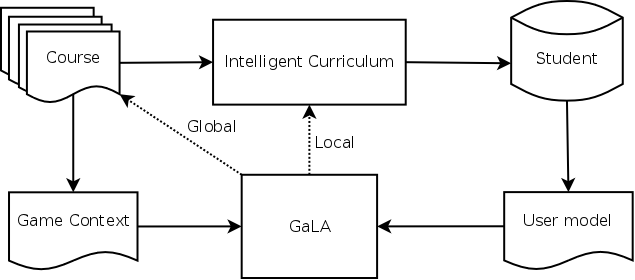
\includegraphics[width=0.9\linewidth]{gala.png}
\caption{The overall architecture of the GaLA system.\label{fig:gala}}
\end{figure}
The overall architecture of GaLA is shown in Figure~\ref{fig:gala}. A course contains a set of learning objects that can transfer various pieces of information in various ways. This set is passed on to a recommender system that selects the best route through the available course materials for a specific student. Such an adaptive route is also known as an intelligent curriculum. The content that is selected by the recommender system is presented to the student, which may result in an increase of the student’s knowledge over time. The knowledge acquired by the student and the measured engagement of a student during the processing of previously offered learning objects is capture in the user model. How this user model is implemented is outside of the scope of this project. This user model serves as one of the two inputs of the GaLA system. The motivational aspects of the learning objects of the course are represented in the earlier described Game Context. This Game Context representation serves as the other 
input of the GaLA system. The GaLA system has as output both local and global recommendations. Global recommendations give feedback to the teacher during course (re)design based on the overall group of students and the average match between the Game Contexts of the available learning objects and the expected (for example based on previous courses) engagement aspects of the user models. The teacher can then try to adapt the course materials in order to on average fit better to the students, of course within the margins of what the teachers finds desirable. In a sense global recommendations try to optimize the engagement globally given the entire group of students. Local recommendations influence the Intelligent Curriculum component directly for a specific student. In a sense the local recommendations try to optimize the engagement locally given the globally defined set of possible learning objects. 

Let’s now look at the workings of the GaLA component more closely. In generic terms, the GaLA system compares the Game Context of each learning object with the engagement evidence from the past given by the User model and combines that into local and global recommendations. The exact instantiation of this generic description depends on the required representations of the recommendations and on the representations of the game context and the engagement evidence. A possible instantiation could be the following setup:
\begin{description}
\item[Game Context] The Game Context of a learning object is represented as an  $n$-dimensional vector containing values for $n$ Game Context elements. These values can either be binaries (present or not present) or reals (gradation of presence).
\item[Engagement evidence] The engagement evidence is a linear regression model that contains the weights for $n$ Game Context elements. These weights indicate how successful the Game Context element seemed to be in triggering engagement based on past experience.
\item[Local recommendations]  Local recommendations are represented as real-valued numbers that indicate how the learning objects are expected to motivate. An intelligent curriculum could take this into account by adopting it as a term in the scoring formula, or the number could be used to choose between several learning objects that contain the same knowledge prerequisites but have different Game Contexts.
\item[Global recommendations] Global recommendations are represented as $n$-dimensional vectors that contains values for $n$ Game Context elements of a specific learning object. These values indicate how much the Game Context element contributed (negatively or positively) to the average student’s engagement. Furthermore it could be displayed as a score for each learning object.
\item[GaLA System] Given the representations of the other components in this example, the GaLA system could calculate local recommendations by linearly combining the weight vectors from the User model with the Game Context of each learning object. For the global recommendations the GaLA System could calculate the average weight vector based on all User models and linearly combined that with each Game Context.
\end{description}

\section{GAMED, Transfer Learning through Game Design}
The user models in GaLA are difficult to create. It is not straight-forward to model the connection between the game elements and the value to be optimized in any given domain. However, the overlap of game elements from different domains is significant as well as that multiple game elements seem to be connected to some higher level element. For instance, a student who is competitive will have higher motivation for competition-related game elements in multiple domains such as gaming and assignments with a competitive nature. If we are able to find a set of higher level elements and how these higher level elements affect, for instance, motivation the task of creating these user models will be easier for new domains. This is a type of transfer learning that can be achieved by finding a set of higher level elements and the connection between that set and the set of game elements in a domain. 

\emph{GAMED} is a system that tries to achieve this type of transfer learning by first finding models that map the game elements in a domain to the value that is being optimized. Once these models have been created for each player in the domain, factor analysis is done on the models to find underlying structure. These values then have to be mapped to the values found on another domain which creates the possibility of estimating a model for another domain.

The first part is to create a model for each individual student. The $n$ game elements in a domain are represented as a vector with $lenght=n$. Since the value that is being optimized is either continuous or a ordered discrete set, the model is created by doing regression. There are a plethora of techniques available to do regression with different properties. For \emph{GAMED}, any of these techniques can be used as long as it remains possible to find the influence of each game element on the higher level variables that are found through factor analysis. 

The models that are created for each person act as user models that map the domain's elements to the value that is optimized. After this has been done for all students, factor analysis is done on the set of user models resulting in a set of higher level variables. The resulting set can then be analysed as to which of the game elements are linked to these higher variables and then compared to a set of these higher variables found for another domain. So the transferring of knowledge from the users in one domain to another is not done automatically. It could be done automatically once enough of these players have user models in both domains so that the mapping between the higher level variables can be found.

% Example
For example, we take the Game Context of the domain of video games and we want to transfer this to the Game Context of the domain of school assignments with respect to their motivational aspects. The first step is to create a user model for each user in the video-game domain. 

An example of how to do this is to track which games a user plays and for how long. For each game, the game elements are given a value as to how important that element is in the game. For each user, a mapping is made between the game element representation and the value for motivation for each game. This value for motivation could be derived from certain other values such as the length of the game session, the frequency with which the game is played and perhaps intensity of play, which can be found by seeing how many badges, or other collectables, the player got during the session. Once the mapping is made for each user, factor analysis is done on all of these models. This results in a set of higher variables which might represent important aspects of the users such as competitiveness.

This is also done for the school assignments domain. Resulting in another set of higher level variables that may represent certain motivational aspects of the users. The difficult part is to find a mapping between these two sets. One method to achieve this would be to create these user models of both domains for a group of users. Then the goal is to find if there is overlap in the higher level variables, which can be done by finding couples of variables that have the same values for all users. Another possibility is to annotate the higher variables using the related game elements and then manually find the mapping between the two sets.

\section{Experiment setup}
The contributions described in this report so far had a theoretical nature. The described Game Context and application areas are based on a review of the literature and brainstorm sessions. This section describes an experiment that was conducted to make a first step in the analysis of the usefulness of the Game Context. In particular the experiment attempts to provide insight in the capabilities of the Game Context to represent engagement in the education domain. 

As mentioned in section \ref{sec:thegamecontext}, each domain has its own set of identifiable game elements. The game elements that the authors found in school assignments are listed in table \ref{tab:game_elements_assignments}.
\begin{table}[ht!]
\centering
\begin{tabular}{ll}
\textbf{Category} & \textbf{Instances} \\ \hline \hline
\emph{Player Configuration} & Single \\
                            & Pair \\
                            & Multi \\ \hline
\emph{Evaluation}           & Final Evalutation \\
                            & Multiple Sub-Evaluations \\
                            & Expert Review \\
                            & Peer Review \\
                            & Relative Grade \\ \hline
\emph{Reward}               & Grade \\
                            & Badges \\
                            & Bonus Content \\
                            & Epic Meaning \\ \hline
\emph{Time Constraints}     & Final Deadline \\
                            & Multiple Deadlines \\
                            & Hard Deadlines \\
                            & Soft Deadlines \\ \hline
\emph{Space}                & Physical Room \\
                            & Virtual Room \\
                            & Isolated \\ \hline
\emph{Assignment Goal}      & Knowledge Acquisition \\
                            & Knowledge Transfer \\
                            & Exploration \\
                            & Consolidation \\
                            & Implementation/Application \\
\end{tabular}
\caption{The game elements discovered in school assignments\label{tab:game_elements_assignments}}
\end{table}
In the experiment, participants were presented with a series of descriptions that they needed to rank on start motivation. The start motivation is defined as the initial motivation that the participants feels to start on the assignment after reading the description. The start motivation was given on a five-point scale (highly demotivated, demotivated, neutral, motivated, highly motivated). The descriptions contained information about a school assignment. These pieces of information were verbalizations of the Game Context elements present in that assignment. For the purpose of the experiment we mapped the found Game Context elements to a set of binary dimensions representing features that are either present or not present (i.e. the opposite feature is present). The binary dimensions and their verbalizations are listed in table \ref{tab:questionnaire_verbalizations}. Besides the set of verbalized gamed context elements that formed the assignment description the participants were also given explanations of each verbalization. These explanations were introduced to prevent any unclarities about the meaning of the verbalizations. The verbalizations and explanations were split up to allow the participant to skip over the explanation part once they familiarized themselves with the concept. The explanations given are listed in table \ref{tab:questionnaire_explanations}.

The descriptions were automatically generated by an algorithm that will now be shortly described. Each description is seen as a bitstring of binary features. The purpose of the algorithm is to get an more or less even distribution of $N$ description points in the multi-dimensional binary space, while keeping overlap between the points. The $N$ descriptions are iteratively generated by mutating from the previous description. The first description is generated by mutating from a bitstring of zeros. Mutation is defined as a fixed number of bitflips at random positions (which may overlap). The mutation is implemented as a mask bitstring that contains 1's at positions that will be flipped. The new description is then obtained by combining the previous description with the mutation mask using the XOR.

The experiment showed participants 20 descriptions, each represented as a bitstring of 9 bits that was generated by flipping 7 bits of the previous description. Participants were furthermore asked in the beginning to enter their current educational program, the year that they are in, their gender, and an indication of their motivation in general on the same five-point scale.

\section{Experiment results}

\begin{table}
  \centering
  \ra{1.3}
  \begin{tabular}{@{}ll@{}}
  \toprule
  Program & Frequency \\ 
  \midrule
  1st year Bachelor Artificial Intelligence & 40 \\
  1st year Master Artificial Intelligence & 41 \\
  1st year Bachelor Computer Science & 27 \\
  3rd year Bachelor Computer Science & 3 \\
  1st year Bachelor Information Science & 2 \\
  3rd year Bachelor Information Science & 2 \\
  2nd year Bachelor Beta-Gamma & 9 \\
  \bottomrule
  \end{tabular}
  \caption{Nicer table format ?}
\end{table}

\begin{table}
  \centering
  \ra{1.3}
  \begin{tabular}{@{}ll@{}}
  \toprule
  Gender & Frequency \\
  \midrule
  Male & 83 \\
  Female & 41 \\
  \bottomrule
  \end{tabular}
  \caption{Nicer table format ?}
\end{table}

\begin{table}
  \centering
  \ra{1.3}
  \begin{tabular}{@{}ll@{}}
  \toprule
  General start motivation & Frequency \\ 
  \midrule
  Highly demotivated & 0 \\
  Demotivated & 0 \\
  Neutral & 52 \\
  Motivated & 72 \\
  Highly motivated & 0 \\
  \bottomrule
  \end{tabular}
  \caption{Nicer table format ?}
\end{table}

\begin{table}\centering
\ra{1.3}
\begin{tabular}{@{}lll@{}}
\toprule
Game Context element & Frequency (present) & Frequence (not present) \\ 
\midrule
Multi Assignment & 53 & 71 \\
Strict deadline & 67 & 57 \\
Bonus & 66 & 58 \\
Badges & 65 & 59 \\
Graded & 60 & 64 \\
Relative grades & 66 & 58 \\
Expert review & 57 & 67 \\
A single final grade & 55 & 69 \\
Group assignment & 61 & 63 \\
\bottomrule
\end{tabular}
\caption{Nicer table format ?}
\end{table}

\clearpage
\section{Analysis of Data}
To better analyse the data, regression is done on the data to find correlation between the game elements and the start motivation. The models that were fitted were linear models that assign a single coefficient to each of the game elements. By analysing these coefficients, it is possible to see what type of impact each game element has on the start motivation. Keep in mind that this does not reveal dependencies between the game elements, but rather views the elements as independent variables. 

The first model is fitted through least median square error regression, resulting in the following coefficients as seen in table \ref{lmsreg}.

\begin{table}[h!t]\centering
\ra{1.3}
\begin{tabular}{@{}llll@{}}
\toprule
\multicolumn{2}{c}{Negative Influence} & \multicolumn{2}{c}{Positive Influence} \\
Game Element & Coefficient &  Game Element& Coefficient  \\ 
\cmidrule(r){1-2}
\cmidrule(r){3-4}
Multiple Assignments 	& -0.0679 	& Graded 		& 0.1635 \\
Strict Deadline 	& -0.0283 	& Expert Review 	& 0.1652 \\
Bonus Content 		& -0.0484 	& Single Final Grade 	& 0.1558 \\
Badges 			& -0.2141 	& Group Assignment 	& 0.0212 \\
Relative Grading 	& -0.1377 	& Default Motivation	& 0.1233\\
\bottomrule
\end{tabular}
\caption{Linear Regression through least median square error}
\label{lmsreg}
\end{table}


The first important conclusion that we can gather is that the data is reasonably well distributed around $0$. Furthermore, some of the coefficients follow what we would expect to see. For instance, strict deadlines result in lower start motivation and multiple assignments also result in lower motivation. Having the grade not counting towards the final grade of the course also results in lower motivation. These three notions follow our initial hypothesis given rise to the notion that the other coefficients may also be good indications of these elements and their impact on motivation.

First, let us look at the elements with a negative impact on motivation. These are:
\begin{itemize}
  \item Badges have the highest negative impact on start motivation
  \item Having a grade relative to other students
  \item Having multiple assignments instead of one final hand-in
  \item Getting access to bonus content
  \item A strict deadline
\end{itemize}

It is rather surprising that badges seem to have a negative impact on start motivation as it is currently a very popular mechanic in the field of gamification. It may be possible that students perceived these badges as resulting in more work, in order to receive the badges, and thus felt less motivated as the entire assignment would be more work. Another possibility is that students feel that the badges do not contribute to their learning experience and that at university level this may affect students.

The same can be said for the bonus content, which was in the form of an extra master class. It may be that the students perceived this as more work, instead of an optional extra.

Another interesting conclusion is that students seem to be negatively influenced by being graded relative to other students. It may be that the students that filled in the questionnaire were less competitive in general. It is also interesting to view this in combination with the negative impact of peer-review. It may be so, that students feel uncomfortable for other students to be able to see their work and to be judged with other students. The social aspects of these two measures may be key to the impact on motivation that the data shows. Being peer-reviewed may also be viewed as being more work, although this was not intended to be the case in the questionnaire.

The elements with a positive impact are as follows:
\begin{itemize}
  \item Being reviewed by the teaching assistant or professor
  \item Having the grade count towards the final grade of the course
  \item Receiving one single final grade instead of multiple grades
  \item Working in groups
\end{itemize}


It is important to note that the positive impact of working in groups is very low and that this may not be indicative of larger groups. It may be so that some students prefer working in groups whilst other prefer working alone. Another possibility is that it does not matter and that students do not feel more or less motivated by either.

Another interesting notion is that being reviewed by the teaching assistant is generally preferred to peer-reviews. However, as noted before, this may be because the students perceive peer-reviews as resulting in more work.

By doing feature selection we can verify the features that have the biggest impact on the start motivation. Feature selection is done using the Aikake measure, resulting in the following coefficients as seen in table \ref{lmsreg_aikake}.

\begin{table}[h!t]\centering
\ra{1.3}
\begin{tabular}{@{}ll@{}}
\toprule
Game Element & Coefficient \\
\midrule
Graded 			& 0.1635 \\
Expert Review 		& 0.1652 \\
Badges 			& -0.2141 \\
Default Motivation	& 0.1233\\
\bottomrule
\end{tabular}
\caption{Linear Regression through least median square error using Aikake measure for feature selection}
\label{lmsreg_aikake}
\end{table}

From these coefficients we can draw the same conclusion that the group of students prefer standard education in the form of grades given by the teaching assistant or professor. Furthermore, this group of students are negatively influenced by the addition of badges.

The model without feature selection had a mean absolute error of $0.7266$ and the model with feature selection had a mean absolute error of $0.7517$. Most of this error is created by the start motivation being on a discrete Likert scale, resulting in regression on a non-continuous scale.

% === Cross-validation ===
% === Summary ===
%  Without Aikake
% Correlation coefficient                  0.2993
% Mean absolute error                      0.7266
% Root mean squared error                  0.9003
% Relative absolute error                 94.0473 %
% Root relative squared error             96.3392 %
% Total Number of Instances              124     

% Time taken to build model: 0 seconds
% 
% === Cross-validation ===
% === Summary ===
% With Aikake
% Correlation coefficient                  0.2687
% Mean absolute error                      0.7517
% Root mean squared error                  0.9018
% Relative absolute error                 97.2939 %
% Root relative squared error             96.4933 %
% Total Number of Instances              124     


\section{Conclusion}
In this report the game context was introduced. The game context is a domain that adheres to three criteria. If a domain has a set of players, a set of mechanics and a set of goals, than the domain can be classified as being a game context. The game context representation is a vector of features which represent the game elements within the domain with respect to the task the game context is created for. Two possible applications were discussed. One of these is GaLA, which is a system that interacts with an intelligent curriculum system by using the game context for both the user models and for representing the course itself. The goal of GaLA is to both give recommendations on a global level to improve the course based on the set of students that will take the course and recommendations on a local level through the intelligent curriculum by giving recommendations to each individual student to facilitate learning.

The other system that was discussed is GAMED, which is a method for transferring knowledge about users from one domain to another. This is done by creating user models in a domain for each individual user. This is followed by finding higher level variables that represent certain aspects that are important to the value which the user models are mapped to. After this, a mapping is made between the higher level variables of multiple domains so that knowledge can be transferred between domains and initial estimates can be given on what aspects might influence a user in another domain.

Both systems were introduced on a conceptual level based on the literature that is currently available for both the domain of gamification and learning analytics. An experiment was done to test whether the game context of a domain captures important aspects of that domain. The experiment was done by using a questionnaire based on the domain of school-assignments. The result of this experiment was that the game context is indeed capable of representing a domain which is not necessarily viewed as being game-like. 


\section{Lessons Learned}
During this research, we ran into several issues which had an impact on the final product. For future research it is important to take the following lessons into account.

\subsection{Current State of Education Data}
% Difficult to gain access to large amounts of data. Learning Record Stores are the solution (?) Sander, write this!

\subsection{User Models}
% Problems with getting unbiased input from users. Especially on the topic of Motivation. How can you better test for motivation


\subsection{Motivational Aspects}
% Motivation may not be prime concern for education. Learning is more important than being motivated or engaged (Although Experiental Flow counters this)

\subsection{Education without Pedagogy}
% Research on Education without adequate study in Pedagogy and Psychology is problematic. We miss these two in our literature, resulting in a lack of theoretical support for the Game Context

\subsection{Current State of Gamification}
As of now, the field of gamification has little academic support. Ample research has been done on motivational or incentive systems, game design and mechanism design.
However, gamification is still in its exploratory phase and most papers published on the subject are applications and qualitative results. This makes it difficult to properly design a system based on gamification. Most work in gamification has been done by commercial institutes which makes it difficult to design new systems from the ground up. It is also difficult to reproduce experiments and there are no standard datasets on which new techniques can be benchmarked.

A large problem is the lack of a proper definition of gamification, apart from the definition by Deterding, resulting in ambiguity as to what actually constitutes as gamification. We used the definition as given by Deterding, but we found that it was not perfect. Therefore, we altered the definition to better describe what game elements are, using literature from the field of game design, and to define game and non-game contexts. This resulted in our definition of a game context, which is different from the usual approach of gamification in which non-game contexts are changed into games by adding game elements. Instead, we defined game contexts to be domains adhering to three criteria. If so, all design patterns within the domain can be viewed as game elements and we use the set which influences a certain external value such as motivation, genre, etcetera.


\pagebreak
\bibliography{literature,literature2}
\bibliographystyle{plain}

\pagebreak
\appendix
\section{Further Possibilities}
\subsection{Looking For Group, an automatic interdisciplinary group forming system}
The first iteration of the game context was just the basic notion that many aspects of education have similar concepts in games. People generally love playing games and experience high motivation and high engagement while doing so, but lack these properties when learning. The idea is that if we rename all education concepts to their respective counterparts in games, we could create a more compelling narrative for the students. This idea is known in the field of gamification as \emph{Epic Meaning} which gives the user the idea that the activity they are doing is much more important. 

When renaming these aspects of education it quickly becomes apparent that the experience itself can be enriched by adding more game elements to learning. When looking at the basic game flow of a course, it seems as though the game itself is fairly simple in structure and the challenge is only provided by the challenge of the course material. The idea is that you can add a new level of challenge on top of the course material, creating a meta-game which provides an easier method to fine-tune the pacing of the challenges and gives students more things to optimize. In modern education, students are mostly concerned with optimizing a single value. One of the reasons for this is that getting a sufficient grade is enough to pass the course and that higher grades do not necessarily matter. 

By adding more dynamic to the course, the students will have more resources to manage and more values to optimize. If correctly designed, this could lead to students spending more time with the course material. 

The idea was to take an interdisciplinary course (Introduction to Game Programming) and renaming all concepts within the course to their counterparts. Students are players, the teacher is the dungeon master, assignments are quests, grades are experience points, the final exam is the boss battle, course materials are weapons/armour/buffs/NPCs.

Since the course is interdisciplinary and focussed on teamwork, it makes sense to view the course as a multiplayer role playing game in which each student chooses a class (vocation) at the start of the course. All activity takes place on an online system where the students have an avatar and a stats-card showcasing their strengths and capabilities.

The classes can be things like game-designers, marketeers, programmers, artists, etc. To do an assignment, or quest, students have to form a group with various classes as required by the assignment. All quests are locked until all participants have reached a high enough level within their class. This results in players having to grind simpler assignments to be able to unlock higher level quests. The idea is that these higher level quests are more interesting, thus motivating students to unlock these quests. 

\subsection{Virtual Economies in the Classroom}

One of the original ideas behind combining learning analytics with gamification was the idea that gamification generates data and is capable of steering behaviour, whilst learning analytics is capable of giving insight into behaviour, making predictions and giving recommendations to students. The idea is that gamification is capable of generating data which can be analysed with learning analytics which in turn can make predictions and give recommendations which can be used to steer the behaviour of the student through gamification. 

The first idea to apply this is by utilizing a model similar to \emph{Stack Overflow}. Stack Overflow is a website meant for programmers to ask questions about certain problems that they face. Other users can respond with their ideas about the subject and are rewarded points for quick responding to questions and users vote on answers so that quality is ensured. This results in a dynamic community where users can go to to resolve issues that they may face. However, more importantly is that Stack Overflow is creating a vast database of problems that programmers might encounter with various solutions to each of them. 

One of the most important skills for programmers is the ability to ask questions and get answers. By allowing students to interact with each other in a stack-overflow-like environment, the students can more easily collaborate on assignments, while also giving the teacher insight into what students are struggling with. One of the main goals is that students are driven to asking better questions, as too simple answers or too complicated or ill-defined questions can be downvoted, resulting in a negative reputation. Students that answer questions quickly and correctly can receive a good reputation on the forum. This also means that the better students will work to give even better answers. Naturally, it is not meant for the students to share answers to the assignments, but a board-moderator (the teaching assistant) can ban students that behave in this manner. This board-like structure will allow students to not get stuck about implementation details and focus more 
on implementing algorithms and structuring code.

In the case of Stack Overflow, points are awarded for responding to questions quickly and by giving good quality answers. This results in that users do not generate content unless there are questions to be answered. Furthermore, in a class-room setting it may be difficult to moderate how much each user relies on the freely available information.

An interesting extension to the Stack-Overflow course, is the possibility of introducing a virtual economy to the classroom. Instead of letting the students freely share answers, it is possible to introduce a currency, called credits, and assigning value to these answers. By viewing answers as knowledge and this knowledge as a product, the students can interact with each other by selling and buying knowledge from each other. Products are valued based on their inherent worth for other students. For instance, the TA could function as an auction-house selling knowledge to the highest bidder. This would allow students who are struggling to use up their credits to make their assignment easier, while good students will work to deliver well structured answers/code to get more credits. All students begin the course with an equal amount of credits, this would make sure that students can’t just buy their way through the course and have to save up credits for when more difficult assignments come. The TA could also 
function as a national bank, making sure there is enough activity on the market and by manipulating the currency. A bank could start buying products, creating more credits, or selling products and thereby lowering the amount of credits in the marketplace. The TA also has to watch over the market as some students may opt to work together and create a cartel in the meantime. 

There are a lot of economic principles that could be introduced and it is unclear how these would affect the classroom. For instance, what would introducing taxes do? Could the bank buy a company/student if that student is sufficiently good? Would a black-market appear and is this unwanted? Could products be in a delayed-release system so that the market works with a slight delay? Could students get loans from the bank and what happens if we introduce rent on these loans? What happens to students that go bankrupt? 


\subsection{Interactive Storytelling in the classroom, non-linear path planning through courses}


\newpage
\section{Questionnaire for GAMED}

\begin{table}
  \centering
  \begin{tabular}{ll|p{0.6\linewidth}}
    \textbf{Game context element} & \textbf{Present} & \textbf{Verbalization} \\ \hline \hline
    Multi assignment & \textbf{false} & All work will be handed in at the end of the assignment \\
    & \textbf{true} & You will hand in multiple sub-assignments \\ \hline
    Strict deadline & \textbf{false} & The deadline is only meant as a guideline and will not be enforced \\
    & \textbf{true} & There is a strict deadline for this assignment \\ \hline
    Bonus & \textbf{false} & (No comment) \\
    & \textbf{true} & Students that perform well can attend a masterclass on the subject \\ \hline
    Badges & \textbf{false} & (No comment) \\
    & \textbf{true} & During the assignment, the TA can give special badges that you can earn for being most creative or most innovative or for best performance \\ \hline
    Graded & \textbf{false} & This assignment is for your own personal benefit and thus the grade for this assignment will not be considered for the final grade of the course \\
    & \textbf{true} & (No comment) \\ \hline
    Relative grades &  \textbf{false} & (No comment) \\
    & \textbf{true} & The assignments will be graded relative to other students \\ \hline
    Expert review & \textbf{false} & Your work will be graded by your fellow students \\
   & \textbf{true} & Your work is graded by the TA \\ \hline
    A single final grade & \textbf{false} & Each individual sub-assignment will be graded \\
    & \textbf{true} & The grade for the assignment is based on the final product \\ \hline
    Group assignment & \textbf{false} & This is an individual assignment \\
    & \textbf{true} & On this assignment you work in groups \\
  \end{tabular}
  \caption{Verbalizations of game context elements in the questionnaire, in both the case where the element is present and where not. The situations that are perceived as default do not have any comments.}
  \label{tab:questionnaire_verbalizations}
\end{table}
\begin{longtable}{ll|p{0.6\linewidth}}
  \textbf{Game context element} & \textbf{Present} & \textbf{Explanation} \\ \hline \hline
  \endfirsthead
  \multicolumn{3}{c}%
  {\tablename\ \thetable\ -- \textit{Continued from previous page}} \\ \hline
  Game context element & Present & Explanation \\ \hline \hline
  \hline
  \endhead
  \hline \multicolumn{3}{r}{\textit{Continued on next page}} \\
  \endfoot
  \hline
  \endlastfoot
  Multi assignment & \textbf{false} & The assignment is handed in as one complete work. However, the assignment may consist of multiple parts that are graded separately \\
  & \textbf{true} & The assignment has multiple moments in which the work so far has to be handed in. This does not mean that each separate assignment is graded \\ \hline
  Strict deadline & \textbf{false} & On this assignment there is not a strict deadline. Naturally, there is a date to hand in your work, but this date is meant as a guideline and it will not be enforced \\
  & \textbf{true} & On this assignment there is a strict deadline. Failing to hand in your work before this deadline also means you fail the assignment and your grade will be modified accordingly \\ \hline
  Bonus & \textbf{false} & (No comment) \\
  & \textbf{true} & By performing well on the assignment, you will get access to some extra content. In this case, the extra content is in the form of a master class given by a famous professor which you can attend \\ \hline
  Badges & \textbf{false} & (No comment) \\
  & \textbf{true} & By achieving certain goals or performing certain tasks you can receive badges. These badges represent things like being the first to hand in the assignment, or getting the best result, being most innovative or creative, being the last to hand it in, doing extra work \\ \hline
  Graded & \textbf{false} & The assignment is not considered in the final computation of your grade for the course. The assignment is still mandatory and you might receive a grade, but the grade is only meant as feedback \\
  & \textbf{true} & (No comment) \\ \hline
  Relative grades &  \textbf{false} & (No comment) \\
  & \textbf{true} & Your grade is based on the performance of other students. For instance, when all students have presented the grades are based on how well other students presented. Another possibility is that the practical is in the form of a competition for which the highest score results in the highest grade \\ \hline
  Expert review & \textbf{false} & This assignment is peer-reviewed which means that your grade is given to you by a fellow student. Naturally this happens under the moderation of the teaching assistant \\
 & \textbf{true} & The grade for this assignment is given by the teaching assistant \\ \hline
  A single final grade & \textbf{false} & This is an assignment that is split up into several smaller assignments or exercises. The smaller assignments are not necessarily handed in separately. For instance, an assignment consisting of multiple exercises for which each exercise is graded \\
  & \textbf{true} & This is a large assignment for which the grade is based on the complete assignment \\ \hline
  Group assignment & \textbf{false} & On this type of assignment you are asked to work alone \\
  & \textbf{true} & On this type of assignment you are asked to work in a group and cooperate on the final product \\
  \caption{Explanations of game context elements in the questionnaire, in both the case where the element is present and where not. The situations that are perceived as default do not have any comments. The explanations are shown at the bottom of the page in addition to the verbalizations.}
  \label{tab:questionnaire_explanations}
\end{longtable}

\end{document}
